\documentclass[border=6pt]{standalone}
\usepackage{tikz}
\usetikzlibrary{arrows.meta}

\definecolor{intfill}{RGB}{233,211,122}    % gold (operators)
\definecolor{leaffill}{RGB}{200,216,242}   % light blue (operands)
\definecolor{nodeline}{RGB}{60,72,140}     % navy edges/outlines
\definecolor{eulercol}{RGB}{200,60,40}     % red Euler-tour curve

\begin{document}
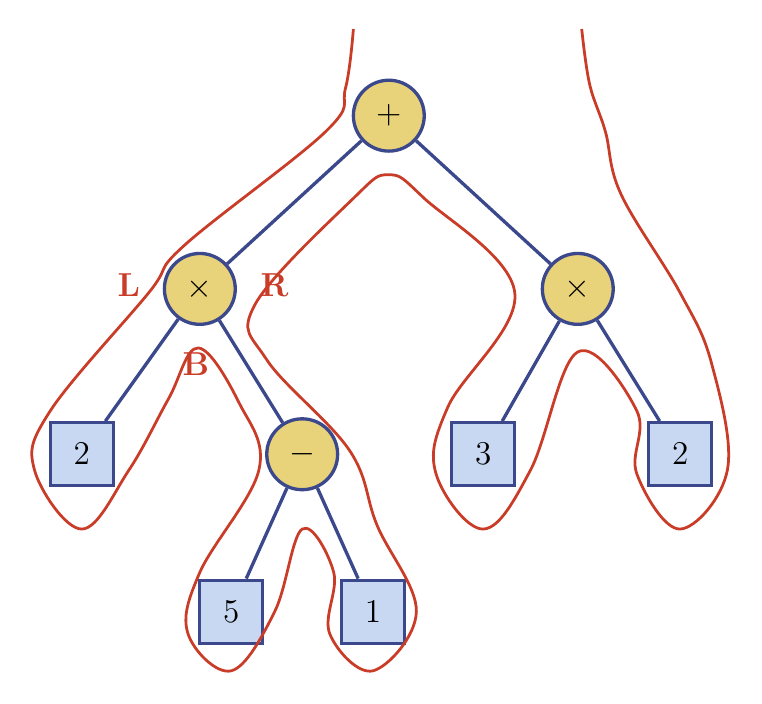
\begin{tikzpicture}[
  op/.style={draw=nodeline, line width=1.2pt, fill=intfill, circle,
             minimum size=9mm, inner sep=0pt, font=\large},
  val/.style={draw=nodeline, line width=1.2pt, fill=leaffill, rectangle,
              minimum size=8mm, inner sep=0pt, font=\large},
  edge/.style={draw=nodeline, line width=1.2pt},
  lbl/.style={text=eulercol, font=\large\bfseries},
]
% ---- Nodes ----
\node[op]  (plus) at (5.0,7.2) {$+$};
\node[op]  (lx)   at (2.6,5.0) {$\times$};
\node[op]  (rx)   at (7.4,5.0) {$\times$};
\node[val] (v2)   at (1.1,2.9) {2};
\node[op]  (minus)at (3.9,2.9) {$-$};
\node[val] (v3)   at (6.2,2.9) {3};
\node[val] (v2b)  at (8.7,2.9) {2};
\node[val] (v5)   at (3.0,0.9) {5};
\node[val] (v1)   at (4.8,0.9) {1};

% ---- Tree edges (drawn under the Euler curve) ----
\foreach \a/\b in {plus/lx, plus/rx, lx/v2, lx/minus,
                   minus/v5, minus/v1, rx/v3, rx/v2b}
  \draw[edge] (\a) -- (\b);

% ---- Euler tour: one continuous curve hugging the tree contour ----
\draw[eulercol, line width=1pt]
  plot[smooth, tension=0.62] coordinates {
    (4.55,8.3) (4.45,7.55) (4.20,7.00) (2.40,5.55) (1.95,4.95)
    (0.70,3.45) (0.50,2.70) (1.10,1.95) (1.70,2.70) (2.20,3.60)
    (2.58,4.25) (3.10,3.55) (3.35,2.70) (2.60,1.40) (2.45,0.62)
    (3.00,0.15) (3.55,0.90) (3.90,1.95) (4.30,1.40) (4.25,0.62)
    (4.80,0.15) (5.35,0.90) (4.85,2.00) (4.50,2.95) (3.45,4.10)
    (3.30,4.80) (4.55,6.15) (5.00,6.45) (5.45,6.15) (6.60,4.95)
    (5.75,3.50) (5.60,2.65) (6.20,1.95) (6.80,2.70) (7.40,4.20)
    (8.15,3.45) (8.15,2.65) (8.70,1.95) (9.30,2.70) (9.10,4.05)
    (8.70,4.95) (7.95,6.20) (7.75,7.00) (7.55,7.60) (7.45,8.30)
  };

% ---- L / B / R encounter labels at the left x node ----
\node[lbl] at (1.70,5.05) {L};
\node[lbl] at (3.55,5.05) {R};
\node[lbl] at (2.55,4.05) {B};
\end{tikzpicture}
\end{document}
